\documentclass[]{article}
\usepackage{lmodern}
\usepackage{amssymb,amsmath}
\usepackage{ifxetex,ifluatex}
\usepackage{fixltx2e} % provides \textsubscript
\ifnum 0\ifxetex 1\fi\ifluatex 1\fi=0 % if pdftex
  \usepackage[T1]{fontenc}
  \usepackage[utf8]{inputenc}
\else % if luatex or xelatex
  \ifxetex
    \usepackage{mathspec}
  \else
    \usepackage{fontspec}
  \fi
  \defaultfontfeatures{Ligatures=TeX,Scale=MatchLowercase}
\fi
% use upquote if available, for straight quotes in verbatim environments
\IfFileExists{upquote.sty}{\usepackage{upquote}}{}
% use microtype if available
\IfFileExists{microtype.sty}{%
\usepackage{microtype}
\UseMicrotypeSet[protrusion]{basicmath} % disable protrusion for tt fonts
}{}
\usepackage[left=3cm,right=3cm,top=2.5cm,bottom=2.5cm]{geometry}
\usepackage{hyperref}
\hypersetup{unicode=true,
            pdftitle={Proposta de procedimento geoestatísticos para a gestão estratégica do atendimento presencial da Receita Federal do Brasil},
            pdfborder={0 0 0},
            breaklinks=true}
\urlstyle{same}  % don't use monospace font for urls
\usepackage{color}
\usepackage{fancyvrb}
\newcommand{\VerbBar}{|}
\newcommand{\VERB}{\Verb[commandchars=\\\{\}]}
\DefineVerbatimEnvironment{Highlighting}{Verbatim}{commandchars=\\\{\}}
% Add ',fontsize=\small' for more characters per line
\usepackage{framed}
\definecolor{shadecolor}{RGB}{248,248,248}
\newenvironment{Shaded}{\begin{snugshade}}{\end{snugshade}}
\newcommand{\AlertTok}[1]{\textcolor[rgb]{0.94,0.16,0.16}{#1}}
\newcommand{\AnnotationTok}[1]{\textcolor[rgb]{0.56,0.35,0.01}{\textbf{\textit{#1}}}}
\newcommand{\AttributeTok}[1]{\textcolor[rgb]{0.77,0.63,0.00}{#1}}
\newcommand{\BaseNTok}[1]{\textcolor[rgb]{0.00,0.00,0.81}{#1}}
\newcommand{\BuiltInTok}[1]{#1}
\newcommand{\CharTok}[1]{\textcolor[rgb]{0.31,0.60,0.02}{#1}}
\newcommand{\CommentTok}[1]{\textcolor[rgb]{0.56,0.35,0.01}{\textit{#1}}}
\newcommand{\CommentVarTok}[1]{\textcolor[rgb]{0.56,0.35,0.01}{\textbf{\textit{#1}}}}
\newcommand{\ConstantTok}[1]{\textcolor[rgb]{0.00,0.00,0.00}{#1}}
\newcommand{\ControlFlowTok}[1]{\textcolor[rgb]{0.13,0.29,0.53}{\textbf{#1}}}
\newcommand{\DataTypeTok}[1]{\textcolor[rgb]{0.13,0.29,0.53}{#1}}
\newcommand{\DecValTok}[1]{\textcolor[rgb]{0.00,0.00,0.81}{#1}}
\newcommand{\DocumentationTok}[1]{\textcolor[rgb]{0.56,0.35,0.01}{\textbf{\textit{#1}}}}
\newcommand{\ErrorTok}[1]{\textcolor[rgb]{0.64,0.00,0.00}{\textbf{#1}}}
\newcommand{\ExtensionTok}[1]{#1}
\newcommand{\FloatTok}[1]{\textcolor[rgb]{0.00,0.00,0.81}{#1}}
\newcommand{\FunctionTok}[1]{\textcolor[rgb]{0.00,0.00,0.00}{#1}}
\newcommand{\ImportTok}[1]{#1}
\newcommand{\InformationTok}[1]{\textcolor[rgb]{0.56,0.35,0.01}{\textbf{\textit{#1}}}}
\newcommand{\KeywordTok}[1]{\textcolor[rgb]{0.13,0.29,0.53}{\textbf{#1}}}
\newcommand{\NormalTok}[1]{#1}
\newcommand{\OperatorTok}[1]{\textcolor[rgb]{0.81,0.36,0.00}{\textbf{#1}}}
\newcommand{\OtherTok}[1]{\textcolor[rgb]{0.56,0.35,0.01}{#1}}
\newcommand{\PreprocessorTok}[1]{\textcolor[rgb]{0.56,0.35,0.01}{\textit{#1}}}
\newcommand{\RegionMarkerTok}[1]{#1}
\newcommand{\SpecialCharTok}[1]{\textcolor[rgb]{0.00,0.00,0.00}{#1}}
\newcommand{\SpecialStringTok}[1]{\textcolor[rgb]{0.31,0.60,0.02}{#1}}
\newcommand{\StringTok}[1]{\textcolor[rgb]{0.31,0.60,0.02}{#1}}
\newcommand{\VariableTok}[1]{\textcolor[rgb]{0.00,0.00,0.00}{#1}}
\newcommand{\VerbatimStringTok}[1]{\textcolor[rgb]{0.31,0.60,0.02}{#1}}
\newcommand{\WarningTok}[1]{\textcolor[rgb]{0.56,0.35,0.01}{\textbf{\textit{#1}}}}
\usepackage{graphicx,grffile}
\makeatletter
\def\maxwidth{\ifdim\Gin@nat@width>\linewidth\linewidth\else\Gin@nat@width\fi}
\def\maxheight{\ifdim\Gin@nat@height>\textheight\textheight\else\Gin@nat@height\fi}
\makeatother
% Scale images if necessary, so that they will not overflow the page
% margins by default, and it is still possible to overwrite the defaults
% using explicit options in \includegraphics[width, height, ...]{}
\setkeys{Gin}{width=\maxwidth,height=\maxheight,keepaspectratio}
\IfFileExists{parskip.sty}{%
\usepackage{parskip}
}{% else
\setlength{\parindent}{0pt}
\setlength{\parskip}{6pt plus 2pt minus 1pt}
}
\setlength{\emergencystretch}{3em}  % prevent overfull lines
\providecommand{\tightlist}{%
  \setlength{\itemsep}{0pt}\setlength{\parskip}{0pt}}
\setcounter{secnumdepth}{0}
% Redefines (sub)paragraphs to behave more like sections
\ifx\paragraph\undefined\else
\let\oldparagraph\paragraph
\renewcommand{\paragraph}[1]{\oldparagraph{#1}\mbox{}}
\fi
\ifx\subparagraph\undefined\else
\let\oldsubparagraph\subparagraph
\renewcommand{\subparagraph}[1]{\oldsubparagraph{#1}\mbox{}}
\fi

%%% Use protect on footnotes to avoid problems with footnotes in titles
\let\rmarkdownfootnote\footnote%
\def\footnote{\protect\rmarkdownfootnote}

%%% Change title format to be more compact
\usepackage{titling}

% Create subtitle command for use in maketitle
\providecommand{\subtitle}[1]{
  \posttitle{
    \begin{center}\large#1\end{center}
    }
}

\setlength{\droptitle}{-2em}

  \title{Proposta de procedimento geoestatísticos para a gestão estratégica do
atendimento presencial da Receita Federal do Brasil}
    \pretitle{\vspace{\droptitle}\centering\huge}
  \posttitle{\par}
    \author{}
    \preauthor{}\postauthor{}
      \predate{\centering\large\emph}
  \postdate{\par}
    \date{17/setembro/2019}

\usepackage{booktabs}
\usepackage{longtable}
\usepackage{array}
\usepackage{multirow}
\usepackage{wrapfig}
\usepackage{float}
\usepackage{colortbl}
\usepackage{pdflscape}
\usepackage{tabu}
\usepackage{threeparttable}
\usepackage{threeparttablex}
\usepackage[normalem]{ulem}
\usepackage{makecell}
\usepackage{xcolor}

\begin{document}
\maketitle

\renewcommand\refname{Referências}

\begin{Shaded}
\begin{Highlighting}[]
\NormalTok{servicos <-}\StringTok{ }\KeywordTok{readRDS}\NormalTok{(}\StringTok{"./dados/02_serviços.rds"}\NormalTok{)}
\NormalTok{viagens <-}\StringTok{ }\KeywordTok{readRDS}\NormalTok{(}\StringTok{"./dados/01_viagens_2.rds"}\NormalTok{)}
\NormalTok{demog <-}\StringTok{ }\KeywordTok{readRDS}\NormalTok{(}\StringTok{"./dados/03_demografia.rds"}\NormalTok{)}
\NormalTok{unids <-}\StringTok{ }\KeywordTok{readRDS}\NormalTok{(}\StringTok{"./dados/04_unidadesRFB.rds"}\NormalTok{) }\OperatorTok\StringTok{ }
\StringTok{        }\KeywordTok{mutate}\NormalTok{(}\DataTypeTok{ibge_unid =} \KeywordTok{ifelse}\NormalTok{(}\KeywordTok{is.na}\NormalTok{(ibge_area), ibge_municipio,  ibge_area)) }\OperatorTok
\StringTok{        }\KeywordTok{distinct}\NormalTok{()}
\end{Highlighting}
\end{Shaded}

\hypertarget{introducao}{%
\section{Introdução}\label{introducao}}

Neste artigo, buscaremos sugerir um processo baseado em dados para
definir uma distribuição eficiente das unidades de atendimento
presencial da Receita Federal do Brasil. Para isso, iremos realizar uma
análise de dados demográficos dos municípios brasileiros, levantado no
Censo de 2010, categorizando-os por proximidade em tempo de viagem de
carro para a unidade de atendimento mais próxima. Com isso, poderemos
descobrir e analisar o público-alvo teórico de cada unidade de
atendimento, descrevendo-os estatisticamente e demonstrando como essa
análise pode ser utilizada para se definir uma reorganização das
unidades atuais.

Na primeira seção, iremos discutir a urgência da aplicação de um método
mais analítico e objetivo na distribuição das unidades de atendimento no
território nacional, levantando obstáculos para a manutenção do
\emph{status quo}. Na segunda seção, explicaremos quais as opções de
modelos geográficos para a efetuação da análise e apontaremos as fontes
de dados que serão utilizadas. Na última seção, realizaremos a descrição
dos públicos-alvo e discutiremos caminhos para expansão, refino e
aplicação prática da análise realizada na tomada de decisão da
organização.

\hypertarget{digitalizacao-crise-e-atendimento}{%
\section{1. Digitalização, crise e
atendimento}\label{digitalizacao-crise-e-atendimento}}

Os recursos, sabemos, são escassos. Frente às necessidades e desejos, a
nobreza do serviço público não subverte tal incômoda realidade. Cabe aos
gestores da coisa pública planejar, executar e controlar o que estiver
sob sua responsabilidade de forma a conhecer a demanda e maximizar a
oferta.

Serviços, diz a definição, são intangíveis: transações que não envolvem
a entrega de bens materiais e conquanto, não assumem uma forma. São
produzidos e consumidos simultâneamente. Hoje, com o advento da internet
e das TIC (tecnologias da informação e da comunicação), é possível
oferecer diversos serviços sem que seja necessária a presença do
ofertante e do demandante no mesmo local físico. O acesso a essas
tecnologias, claro, ainda é limitado.

Este é o caso do atendimento presencial oferecido por diversos órgãos
públicos, conjunto no qual está inserida a Secretaria da Receita Federal
do Brasil (RFB). Por ele, o cidadão pode tanto entregar quanto
requisitar informações, declarações e documentos essenciais à
conformidade tributária, auxiliando no papel da instituição de recolher
os recursos necessários ao provimento dos diversos serviços públicos
oferecidos pelo Estado brasileiro. No papel de orientação, são também
instrumentos de educação fiscal e promoção da auto-regularização,
fomentando uma cultura de conformidade pro-ativa e cidadã.

O atendimento já foi alvo de extensa digitalização, evidenciado em seus
números. A virtualização dos serviços de atendimento da RFB avança a
passos largos; entre 2012 e 2017, o e-Cac, portal de atendimento na
internet da RFB, passou de 66,6 milhões de atendimentos para 145,6
milhões de atendimentos. Enquanto isso, os atendimentos presenciais
caíram de 20,2 milhões para 14,9 milhões no mesmo período, de forma que
o percentual destes passou de cerca de 24\% do total para apenas 9\%
({\textbf{???}}). Mesmo assim, 14,9 milhões equivalem a 40.000 cidadãos
recebidos nas 522 unidades da RFB por dia, em todo o país.

Desta realidade, surgem os dilemas do gestor. Para suprir essa
necessidade de simultaneidade física entre os servidores da RFB e o
cidadão demandando serviços, cabe a ele escolher como distribuir
geograficamente os recursos materiais e os servidores disponíveis.

Estes dilemas não tem solução única. Possíveis respostas tem sido
levantadas em outros setores de serviço, como de transporte e de saúde,
com a aplicação de Sistemas de Informações Geográficas (GIS, na sigla em
inglês) e técnicas de geoestatísticas que permitam encontrar soluções
numericamente satisfatórias. No exemplo do setor de saúde, por exemplo,
o problema é exposto da seguinte forma:

\begin{quote}
``os serviços de saúde são providos em um número finito de locais fixos,
todavia, servem populações que estão distribuídas de forma contínua e
desigual por uma região (Delamater et al. 2012, 1).''\footnote{``health
  care services are provided at a finite number of fixed locations, yet
  they serve populations that are continuously and unevenly distributed
  throughout a region''.}
\end{quote}

Consequência natural desse arranjo é que as desigualdades são
inevitáveis, mas a dimensão dessas é função: do arranjo de distribuições
das partes do sistemas; da distribuição no espaço da população; e das
características do espaço, como infraestrutura e relevo, que dificultem
ou facilitem a movimentação (Delamater et al. 2012).

Ao se analisar a relação entre população e o espaço físico, podemos
evidenciar a resistência ao acesso de diferentes grupos populacionais,
aos serviços identificar áreas de maior limitação no acesso, e, assim,
``compreender o efeito de se abrir, fechar ou realocar unidades de saúde
(Delamater et al. 2012, 2).''\footnote{``understand the effects of
  opening, closing, or realocating health care facilities''.} Desta
forma, promove-se a equidade, que ``(\ldots{}) se manifesta na
distribuição, acesso e utilização de serviços de saúde entre grupos da
população (Noor et al. 2003, 917).''\footnote{``(\ldots{}) manifests
  itself in the distribution, access to and utilization of health
  services between population groups''.}

A relevância da distribuição ótima é tanto mais importante quanto mais
escassos forem os recursos disponíveis. O Brasil enfrenta desde meados
de 2014 uma grave crise econômica, com efeitos diversos sobre a
população e sobre a estrutura administrativa do Estado. Mesmo o órgão
arrecadador não escapa das restrições necessárias ao ajuste fiscal
aplicado na tentativa de debela-la. Neste sentido, o TCU, em auditoria
operacional realizada na RFB, relata que

\begin{quote}
``além da crise econômica que o País vem enfrentando, que impacta a
receita fazendária e a previdenciária, tem-se constatado a ocorrência de
baixa recuperação dos créditos trbutários administrados pela RFB''
(Contas da União 2017, 1).
\end{quote}

Os reflexos internos na Receita Federal do Brasil são o
contingenciamento de despesas e a paralisação de concursos, estancando o
fluxo de renovação de servidores. Em paralelo, há um processo de
aceleração nas aposentadorias, muitas delas influenciadas pelo temor que
os anúncios da reforma previdenciária inspiram.

Vale lembrar que muitos servidores na ativa já alcançaram o requisito
mínimo para aposentar-se mas continuam em serviço, incentivados pelo
chamado abono permanência (Contas da União 2017). Entre 2015 e 2017, a
RFB perdeu 1.831 servidores, de um total inicial de 23.687, o que
representa uma diminuição de 7,7\% de sua força de trabalho em apenas 3
anos.

Este enxugamento, pode-se argumentar, não seria de todo impactante na
organização, posto que, com o avançar da digitalização, haveria um
aumento na produtividade que compensaria em parte ou mesmo totalmente os
efeitos da diminuição na quantidade de servidores. Todavia, lembra o TCU
que

\begin{quote}
``(\ldots{}) não se pode contar apenas com a evolução dos meios de
tecnologia da informação, pois os mesmos dependem de fatores exógenos
como questões orçamentárias, disponibilidade do Serpro para
desenvolvimento de sistemas e outros que não permitem sua evolução com
velocidade o suficiente para suprir a nova demanda'' (Contas da União
2017, 20).
\end{quote}

Desta forma, temos todos os fatos em frente aos gestores da Receita
Federal do Brasil. De um lado, há um quantitativo decrescente de
servidores disponíveis para as tarefas da organização. De outro,
percebemos uma gama de obstáculos que impossibilitam sua substituição
imediata por canais digitais. Cabe-os então decidir, como distribuir as
unidades da forma mais eficiente? De que maneira promover a equidade no
acesso aos serviços da organização? O objetivo do presente trabalho é
sugerir um modelo que, incluído num processo maior, possa responda às
essas necessidades.

Acreditamos que esse processo de distribuição das unidades de
atendimento está no âmago da estratégia da Receita Federal do Brasil e
de seu propósito para a sociedade. Como tal, sugerimos que, definidas as
balizas estratégicas de qual público alvo deve ser atingido pelas
unidades de atendimento, a organização empregue modelos geoestatísticos
na tomada de decisões de que unidades abrir e fechar e quantos
servidores devem se dedicar em cada unidade, de acordo com a demanda
estimada para cada ponto geográfico. Desta forma, a distribuição estaria
mais alinhada ao seu objetivo social, tornando-o menos vulnerável a
captura política.

Este trabalho, de forma mais pontual, busca mostrar a viabilidade do
cruzamento de dados estatísticos e geoestatístico do IBGE e de outras
fontes para conhecer e explorar informações relevantes sobre o público
alvo das unidades de atendimento, um dos passos necessários ao processo
descrito acima.

Antes de passarmos a sua execução, cabe ressalva importante. Embora a
disponibilidade e a distância sejam fatores relevantes, não são
suficientes; o aumento da acessibilidade nem sempre é acompanhado de um
aumento da utilização dos serviços, e outros fatores devem ser avaliados
também, como qualidade do serviço oferecido e disponibilidade de canais
mais convenientes (Thaddeus and Maine 1994), como os próprios canais
digitais supracitados. Que fique claro que a definição de onde dispor
unidades de atendimento é apenas um passo do objetivo estratégico de
atender bem a população.

\hypertarget{das-fontes-de-dados-e-metodos-de-extracao-analise-e-cruzamento}{%
\section{2. Das fontes de dados e métodos de extração, análise e
cruzamento}\label{das-fontes-de-dados-e-metodos-de-extracao-analise-e-cruzamento}}

\hypertarget{mapas-vetoriais-e-mapas-em-grade}{%
\subsection{2.1 Mapas vetoriais e mapas em
grade}\label{mapas-vetoriais-e-mapas-em-grade}}

Há duas formas de se dispor dados em sistemas de informação geográficas.
Há os modelos vetoriais, que podem ser analisados como grafos em redes (
\emph{network graphs} ); e os modelos em grade ( \emph{raster} ).

Os modelos vetoriais consistem de uma série de nós, conectados por
linhas, representando os objetos geográficos. Pontos no mapa são
representados por nós; conexões e infraestruturas como ferrovias e
rodovias são linhas, e regiões são delimitadas por polígonos, nós
combinados com vértices. Nos modelos vetoriais, o custo para atravessar
uma linha é função do tamanho da linha e da velocidade de viagem
associado àquele tipo de infraestrutura (Delamater et al. 2012). a
movimentação, portanto, ocorre entre pontos, de acordo com as linhas
disponíveis para cada ponto.

Os modelos de grade são compostos por uma série de celulas regulares,
geralmente retangulares, de tamanho e distância padronizados. Cada ponto
do mapa é resumido em um dos retângulos, e todas as informações
relevantes do mapa dentro da região encoberta por aquele retângulo são a
ele atribuído. No modelo de grade, as viagens ocorrem na passagem de uma
célula para outra, sempre em entre células adjacentes; assim, diferente
do modelo em rede, os passos da viagem são sempre regulares em
distância, variando apenas na velocidade (Delamater et al. 2012).

Vemos acima uma conversão entre um mapa em network para um mapa em grid
(Delamater et al. 2012, fig. 12). Há uma diferença fundamental na forma
como esses modelos compreendem o espaço.

\begin{quote}
``O modelo de dados em grade define o espaço como uma superfície
contínua onde cada célula do espaço dos dados tem um local específico e
um valor de atributo. O modelo de dados em rede define o espaço como um
recipiente vazio populado apenas pelas características de locais e
atributos específicos (Delamater et al. 2012, 12).''\footnote{``The
  raster data model defines space as a continuous surface where each
  cell within the data extent has a specific location and attribute
  value. The network data model defines space as an empty container that
  is populated only by features having specific locations and
  attributes.''}
\end{quote}

Como todas as localizações do mapa são explicitamente definidadas nos
modelos de grade, isso torna-os ``(\ldots{}) atraentes para criação de
áreas de serviço, especialmente em regiões sem redes de transporte
abrangentes (Delamater et al. 2012, 4).''\footnote{``(\ldots{})
  attractive for creating service areas, specially in regions without a
  all-encompassing transportation network''} Todavia, ``conectividade na
vida real não é levada em consideração nos modelos de dados em grade
(\ldots{}), portanto, o movimento é menos restringido nos modelos de
dados em grade do que no mundo real e as estimativas de tempo de viagem
vão ser geralmente subestimadas (Delamater et al. 2012, 15)''.\footnote{``real-world
  connectivity is not accounted for in the raster data model (\ldots{})
  therefore, movement is less restricted in the raster data model than
  in the real world and travel time estimates will generaly be
  underestimated''}

Isso ocorre porque o modelo considera que todos os pontos do mapa são
atravessáveis, fazendo, por exemplo, que um viajante pudesse
aproveitar-se da infraestrutura ferroviária entrando em qualquer ponto
que fosse mais próximo dele, ignorando a existência de estações ou, no
caso de rodovias, intersecções (J. Weiss et al. 2018).

Para nós, a adoação de um modelo vetorial bastaria para uma primeira
aproximação. O modelo em grade enfrentaria as limitações mencionadas
acima e seu custo computacional seria consideravelmente mais elevado.
Ademais, o modelo em grade serviria apenas para as poucas regiões do
país com baixa densidade de infraestrutura.

Inicialmente, havíamos considerado a utilização de informações de
infraestrutura do Malaria Atlas Project para estimar o custo de fricção,
que foi gerado a partir de informações obtidas do Open Street Map (J.
Weiss et al. 2018). Optamos, todavia, pela utilização direta dos dados
do Open Street Map, simplificando os municípios para pontos unitários no
espaço geográfico.

Algumas presunções devem ser explicitadas antes de qualquer análise.
Primeiro, os modelos assumem que todos possuem acesso a veículos
similares e que se movimentam nesses veículos de forma similar, o que
pode ser pouco realista mesmo considerando-se apenas viagens terrestes.
``A riqueza em particular é um determinante provável de se alguém irá
viajar à pé em vez de tomar um véiculo e, portanto, afeta
substancialmente a acessibilidade no nível do indivíduo (J. Weiss et al.
2018, 338).''\footnote{``Wealth, in particular, is a likely determinant
  of whether someone travels on foot rather than taking a vehicle and
  thus substantially affects acessibility on the level of the
  individual''}

Em segundo lugar, assume-se uniformidade nas condições de viagem,
ignorando-se horário, sazonalidades como horário de rush ou fins de
semana e feriados, variações temporais e climáticas, etc. Em terceiro
lugar, assume-se que as pessoas conhecem o caminho mais eficiente; uma
presunção razoável atualmente, com o amplo acesso à sistemas de
navegação em celulares e computadores. Em quarto lugar, presume-se que
as populações concentram-se num único ponto; ou seja, qualquer variação
da distribuição interna a cada um dos retângulos da grade é ignorada, e
atribui-se à centroide de cada retângulo a totalidade da população
daquele espaço (Delamater et al. 2012).

Seria mais realista um modelo que pudessemos combinar as informações
demográficas dos grupos populacionais mais próximos, independente de
divisões municipais. Todavia, esse tipo de levantamento de dados não
seria apenas custoso mas também traria diversos riscos à privacidade da
população analisada. Como tal, fazemos o registro apenas para reconher o
risco, em nossa análise, de enfrentarmos algumas falácias estatísticas,
como a falácia ecológica e o problema da unidade de área modificável.

\hypertarget{download-e-preparacao-dos-dados}{%
\subsection{2.2 Download e preparação dos
dados}\label{download-e-preparacao-dos-dados}}

Para realizar as analises propostas, uma gama de fontes de dados de
natureza e informações diferentes foram levantadas. As informações
levantadas foram:

\begin{enumerate}
\def\labelenumi{\arabic{enumi}.}
\tightlist
\item
  Serviços de atendimento disponibilizados pela Receita Federal do
  Brasil, tanto digitalmente quanto presenciais
\item
  Unidades de atendimento da RFB em funcionamento, com endereço e tipo
  de unidade, de acordo com a estrutura organizacional
\item
  Malha digitais dos municípios brasileiros presentes no Censo 2010
\item
  Tabelas agregadas de população economicamente ativa e inativa e de
  população por faixa etária em cada um dos municípios presentes no
  Censo 2010
\item
  Malha digitais das áreas de ponderação presentes no Censo 2010,
  restritas aos municípios de São Paulo, Rio de Janeiro, Belo Horizonte
  e Curitiba
\item
  Tabelas agregadas de população economicamente ativa e inativa e de
  população por faixa etária em cada uma das áreas de ponderação
  mencionadas no Censo 2010
\item
  Duração e tempo de viagem à carro entre todos os municípios e áreas de
  ponderação mencionadas acima
\end{enumerate}

Primeiramente, foram levantados os serviços disponíveis na Receita
Federal, para descobrirmos quais dos serviços oferecidos necessitam do
canal presencial das unidades de atendimento. Essas informações foram
extraídas diretamente do site da RFB na internet. Outra informação
obtida no site da Receita foi a lista atualizada de unidades de
atendimento disponíveis, incluindo seus endereços e tipos.

Para efetuas essas extrações, utilizamos o pacote RSelenium rodando em
um container Docker, para garantir uma extração rápida e fácil de ser
reproduzida. Um container é uma unidade padrão de software que empacota
um código e todas a suas dependências, rodando-o de forma consistente e
rápida, e muito mais leve do que se fosse criada toda uma máquina
virtual para a tarefa
(\url{https://www.docker.com/resources/what-container}). Esse esquema
foi necessário porque, infelizmente, essas informações ou não estão
disponibilizadas como Dados Abertos pela RFB, ou estão desatualizadas.

Com os dados das unidades de atendimento e dos serviços, uma escolha
pode ser realizada. Percebemos que, em geral, há uma divisão muito clara
entre serviços de atendimento de natureza aduaneira e serviços de
natureza tributária; ademais, para as pessoas físicas, os serviços
aduaneiros resumem-se àqueles de verificação de bagagem internacional.
Essas descobertas são melhor desenvolvidas na seção 3.1, abaixo.

Ademais, quando restringimos as unidades de atendimento àquelas que
prestam serviços de natureza tributária, percebemos também que elas, em
geral, resumem-se a apemas uma unidade por municópio, com exceção dos
municípios de São Paulo, Rio de Janeiro, Belo Horizonte e Curitiba.

Com essa informação em mãos, decidimos que a localização geográfica
exata das unidades de atendimento, em geral, não nos interessava;
bastava-nos saber que eles estavam localizados num município, e
poderíamos utilizar a localização do município, registrado em banco de
dados fornecido pelo IBGE, como localização da unidade, com baixa margem
de erro nos cálculos de tempo de viagem entre os outros municípios e
aquela unidade.

A exceção se deu nos quatro municípios citados. Para essas unidades,
decidimos ir ao nível de área de ponderação, subdivisão censitária
estabelecida pelo IBGE. Por isso, precisávamos da localização de cada
unidade de atendimento destes municípios para identificar a qual área de
ponderação ela estava contida. Para isso, utilizamos a API do Google
Maps, que, a partir do endereço extraído no site da RFB, nos devolvia
uma coordenada geográfica que podíamos utilizar para definir a área de
ponderação que a continha.

As malhas digitais dos municípios foram obtidas no IBGE. As malhas dos
municípios puderam ser obtidas sem grandes dificuldades utilizando o
pacote GeoBr, disponibilizado no GitHub pelo IPEA; as malhas das áreas
de ponderação, todavia, não puderam ser obtidas com o mesmo pacote,
devido à problemas no código desse; baixamos as malhas dos setores
censitários, disponibilizadas em FTP pelo IBGE, e utlizando informação
entregue pelo IBGE em consulta de SAI, fizemos o agrupamento dos setores
nas áreas de ponderação.

Para os municípios e áreas de ponderação em análise, obtivemos no IBGE
tabelas do censo que nos dessem informações sobre a população
economicamente ativa e inativa e sobre a distribuição da popílação por
faixa etária, além da distribuição por faixa salarial. Para os
municípios, essas informações vieram da Tabela 616 - Pessoas de 10 anos
ou mais de idade por grupos de idade, condição de atividade na semana de
referência, sexo e situação do domicílio e da tabela 1384 - Pessoas de
10 anos ou mais de idade, por classes de rendimento nominal mensal -
Universo. Das áreas de ponderação, vieram das tabelas 1572 - Pessoas de
10 anos ou mais de idade, por idade e condição de atividade e de
ocupação na semana de referência - Resultados Gerais da Amostra e 2030 -
Pessoas de 10 anos ou mais de idade, por classes de rendimento nominal
mensal - Resultados Gerais da Amostra.

Por fim, as informações de tempos e distâncias de viagem à carro entre
os municípios. Útilizamos os dados disponibilizados gratuitamente no
OpenStreetMap para fazer essas medições. Devido ao volume de dados
vetoriais que servem de insumo a essas estimativas, além do número de
cruzamentos diferentes, na casa dos 4 milhões, nós tivemos que montar um
servidor local que pudesse processar esse número de operações.
Utilizamos novamente um container docker, mas dessa vez, nós o montamos
dentro de uma instância computacional virtual, utilizando os serviços do
Google Cloud Platform. Todos esses dados processados estão disponíveis
publicamente, via Dropbox, nas urls abaixo:

\begin{itemize}
\tightlist
\item
  \href{https://www.dropbox.com/s/jkiiwwxz73eys9e/01_viagens.rds?raw=1}{Arquivo
  RDS com informações dos tempos e distâncias de viagens}
\item
  \href{https://www.dropbox.com/s/84hrt2ntrx9k0t0/02_servi\%C3\%A7os.rds?raw=1}{Arquivo
  RDS com informações dos serviços prestados pela Receita Federal do
  Brasil}
\item
  \href{https://www.dropbox.com/s/stsxm0cl98lmnzg/03_demografia.rds?raw=1}{Arquivo
  RDS com informações demográficas de municípios e áreas de ponderação
  selecionados}
\end{itemize}

\hypertarget{dos-resultados}{%
\section{3. Dos resultados}\label{dos-resultados}}

\hypertarget{potencial-digital-dos-servicos-da-rfb}{%
\subsection{3.1 Potencial digital dos serviços da
RFB}\label{potencial-digital-dos-servicos-da-rfb}}

A principal limitação à plena digitalização dos serviços da Receita
Federal está na necessidade de autenticação digital dos cidadãos. Devido
à sensibilidade dos serviços da RFB, que envolvem tanto informações
sensíveis da vida financeira e da identidade da pessoa, como também
envolvem impactos financeiros, é necessário utilzar certificados
digitais para a maioria dos serviços online.

O certificado digital é uma assinatura eletrônica com criptografia para
confirmar a identidade de uma pessoa física (e-CPF) ou empresa (e-CNPJ).
Ele possui poder jurídico e contém dados do titular como nome, registro
civil e assinatura da autoridade certificadora, e pode custa de cerca de
100 reais até 400 reais por ano, dependendo do segmento e do tipo do
certificado
(\url{https://nfe.io/blog/assinatura/quanto-custa-certificado-digital/}).

Devido ao alto custo, o número de pessoas físicas com certificado
digital é pequeno; por outro lado, a obrigatoriedade legal da posse de
certificados digitais para pessoas jurídicas está se expandindo ano a
ano, e por isso, os serviços presenciais de pessoas jurídicas na RFB
está em franco declínio, restando às unidades atenderem as pessoas
física. As empresas, em sua massiva maioria, já possuem certificado
digital, se não por necessidade, mas por obrigação legal, que está se
extendendo progressivamente aos CNPJs de menor faturamente. Em julho de
2018, por exemplo, passou a ser obrigatório para pequenas empresas.
Desta forma, podemos nos concentrar nos serviços prestados ao cidadão,
listados 253 nessa página da internet.

É possível que, no futuro, a RFB adote outras formas mais simples e
baratas de autenticação do cidadão, expandindo os acessos digitais a
seus serviços. Um exemplo é o login único do governo federal, que está
sendo lentamente adotado por diversos órgão da União
(\url{http://faq-login-unico.servicos.gov.br/en/latest/_perguntasdafaq/oquee.html}).
Até lá, as unidades presenciais servirão como canal de complementação
àqueles que não possuírem os meios para acessar os serviços digitais.

Pois bem, podemos então nos perguntar, que serviços não estão
digitalizados e, como tal, a resolução do problema do certificado
digital não bastaria para que deixassem de ser realizados em unidades de
atedimento? Pelas razões já citadas, iremos nos ater aos serviços ao
cidadão, e não às empresas, como listados no site da Receita Federal.

\begin{Shaded}
\begin{Highlighting}[]
\CommentTok{#servicos <- readRDS(url('https://www.dropbox.com/s/84hrt2ntrx9k0t0/02_servi%C3%A7os.rds?raw=1'))}
\KeywordTok{nrow}\NormalTok{(servicos)}
\end{Highlighting}
\end{Shaded}

\begin{verbatim}
## [1] 253
\end{verbatim}

Alguns dos serviços desta lista se misturam com os serviços às empresas,
posto que podem ser fornecidos aos dois. Em geral, um serviço que se
presta a uma empresa mas também pode ser prestado a um cidadão é
fornecido desta maneira simplesmente para não criar obstáculos
desnecessários àqueles que ainda não tenham um CNPJ. Na prática, são
serviços exclusivos para CNPJs, que, por desburocratização, podem ser
prestados a alguém que não o tenha em mão. Por isso, para saber quais os
serviços criados com foco nas pessoas físicas, devemos filtrar essa
lista.

\begin{Shaded}
\begin{Highlighting}[]
\NormalTok{eval02 <-}\StringTok{ }\NormalTok{servicos }\OperatorTok\StringTok{ }\KeywordTok{filter}\NormalTok{(publico_alvo }\OperatorTok\StringTok{ }\KeywordTok{c}\NormalTok{(}\StringTok{"Pessoa Física"}\NormalTok{))}
\KeywordTok{nrow}\NormalTok{(eval02)}
\end{Highlighting}
\end{Shaded}

\begin{verbatim}
## [1] 60
\end{verbatim}

Resta-nos portanto, 60 serviços prestados pela Receita Federal a pessoas
físicas, ou seja, a pessoas que não são obrigadas a possuir e, como
discutido, provavelmente não possuem certificados digitais. Diversos
desses serviços tem o canal digital, portanto, como opcional. Se a
pessoa possuir o certificado digital, ela pode acessar um canal
eletrônico da Receita (geralmente mas nem sempre o e-Cac), mas, se não
possuir, pode se dirigir a uma unidade de atendimento.

Assim, para responder a pergunta de quantos serviços são exclusivamente
presenciais, temos que filtrar essa lista mais ainda, para os serviços
que não possuem qualquer opção de canal eletrônico.

\begin{Shaded}
\begin{Highlighting}[]
\NormalTok{eval03 <-}\StringTok{ }\NormalTok{servicos }\OperatorTok\StringTok{ }
\StringTok{            }\KeywordTok{filter}\NormalTok{((tipo_atendimento }\OperatorTok\StringTok{ }\KeywordTok{c}\NormalTok{(}\StringTok{"Atendimento pela internet"}\NormalTok{, }\StringTok{"Atendimento e-CAC"}\NormalTok{))) }\OperatorTok
\StringTok{            }\KeywordTok{filter}\NormalTok{(publico_alvo }\OperatorTok\StringTok{ }\KeywordTok{c}\NormalTok{(}\StringTok{"Pessoa Física"}\NormalTok{)) }\OperatorTok\StringTok{ }
\StringTok{            }\KeywordTok{select}\NormalTok{(nome, tipo_atendimento)}
\NormalTok{eval04 <-}\StringTok{ }\NormalTok{servicos }\OperatorTok\StringTok{ }
\StringTok{            }\KeywordTok{filter}\NormalTok{(}\OperatorTok{!}\NormalTok{(tipo_atendimento }\OperatorTok\StringTok{ }\KeywordTok{c}\NormalTok{(}\StringTok{"Atendimento pela internet"}\NormalTok{, }\StringTok{"Atendimento e-CAC"}\NormalTok{))) }\OperatorTok
\StringTok{            }\KeywordTok{filter}\NormalTok{(publico_alvo }\OperatorTok\StringTok{ }\KeywordTok{c}\NormalTok{(}\StringTok{"Pessoa Física"}\NormalTok{)) }\OperatorTok\StringTok{ }
\StringTok{            }\KeywordTok{left_join}\NormalTok{(eval03, }\DataTypeTok{by=}\KeywordTok{c}\NormalTok{(}\StringTok{"nome"}\NormalTok{)) }\OperatorTok
\StringTok{            }\KeywordTok{filter}\NormalTok{(}\KeywordTok{is.na}\NormalTok{(tipo_atendimento.y)) }\OperatorTok\StringTok{ }
\StringTok{            }\KeywordTok{select}\NormalTok{(nome}\OperatorTok{:}\NormalTok{descricao)}

\KeywordTok{kable}\NormalTok{(eval04) }\OperatorTok
\StringTok{  }\KeywordTok{kable_styling}\NormalTok{(}\DataTypeTok{bootstrap_options =} \KeywordTok{c}\NormalTok{(}\StringTok{"striped"}\NormalTok{, }\StringTok{"hover"}\NormalTok{))}
\end{Highlighting}
\end{Shaded}

\begin{table}[H]
\centering
\begin{tabular}{l|l|l}
\hline
nome & nome\_popular & descricao\\
\hline
Bagagem - Tratamento Tributário & Bagagem & Orientações acerca do conceito e do tratamento tributário de bagagem.\\
\hline
Bagagem Acompanhada & Bagagem acompanhada & Apresentação da declaração de bagagem acompanhada.\\
\hline
Bagagem Acompanhada - Cálculo do Imposto e emissão do DARF & Bagagem Acompanhada & Solicitar o cálculo do Imposto de Importação e a emissão de Darf para bagagem acompanhada.\\
\hline
Habilitação - Pessoa Física & NA & Solicitar habilitação da pessoa física para importar e/ou exportar.\\
\hline
Concluir o Serviço no CPF que gerou protocolo de atendimento & NA & Concluir o pedido de inscrição, alteração ou regularização no CPF cuja solicitação foi iniciada em um conveniado (Ex: Banco do Brasil, Caixa, Correios e outros) e gerou um protocolo de atendimento não conclusivo.\\
\hline
Realizar Serviços no CPF - Falecidos & NA & Solicitar atendimento em unidade da Receita Federal para inscrição, alteração, regularização e cancelamento no CPF de pessoa falecida.\\
\hline
DIRPF - Solicitar Cancelamento & NA & Solicitar o cancelamento da declaração do IRPF, a partir do exercício de 2008.
É possível solicitar o cancelamento da DIRPF nas seguintes situações:
A pedido do contribuinte, desde que não sejam identificados indícios de fraude, informando o motivo do cancelamento da declaração entregue.
Quando o contribuinte não reconhecer a DIRPF entregue e alegar fraude ou falsidade.\\
\hline
Incluir/Excluir o Nome Social no CPF & NA & Incluir/excluir no cadastro de pessoa física o nome pela qual a pessoa travesti ou transexual é socialmente reconhecido e que constará no comprovante de inscrição e no comprovante de situação cadastral do CPF.\\
\hline
\end{tabular}
\end{table}

Como podemos conferir, dos 253 serviços iniciais, apenas oito se
encaixam nessa lista restrita. Três deles se referem a casos específicos
de tratamento de CPF, um se refere a habilitação aduaneira de pessoa
física, três se referem ao tratamento de bagagem para viajantes
internacionais e um a possibilidade de cancelamento do imposto de renda.
Como tal, com exceção óbvia dos serviços de análise de bagagens em
viagens internacionais, realizadas na descida do avião de passageiro de
vôo internacional, parece-nos pouco provável que esses serviços
escapariam à digitalização.

Portanto, o que concluímos disso é que a necessidade das unidades
presenciais se deve muito menos à inexistência de canais digitais e
muito mais à dificuldade de se conceder acesso seguro e barato à
população nesses canais.

\hypertarget{publico-alvo-da-unidades-de-atendimento-da-receita-federal-do-brasil}{%
\subsection{3.2 Público-alvo da unidades de atendimento da Receita
Federal do
Brasil}\label{publico-alvo-da-unidades-de-atendimento-da-receita-federal-do-brasil}}

Posto que o problema dos certificados digitais não está resolvido,
resta-nos analisar as unidades de atendimento existentes. A análise que
faremos será de buscar qual o público-alvo hipotético de cada unidade de
atendimento da Receita Federal.

Nós estamos definindo público alvo de uma unidade de atendimento como
toda a população dos municípios para os quais é mais rápido, em tempo de
viagem, chegar à aquela unidade de atendimento do que a qualquer outra
unidade de atendimento disponível.

Nós dizemos que é hipotético porque, como discutido nas ressalvas finais
da seção 1, o tempo de viagem e a distância não são os únicos fatores a
definirem para onde o cidadão vai escolher ser atendido. Ainda assim,
acreditamos ser dos fatores mais importantes, e por isso, uma boa
primeira aproximação.

\begin{Shaded}
\begin{Highlighting}[]
\CommentTok{# usar dados de viagens para, para cada município, descobrir a unidade de atendimento mais próxima}
\CommentTok{#viagens <- readRDS(url("https://www.dropbox.com/s/jkiiwwxz73eys9e/01_viagens.rds?raw=1"))}
\CommentTok{#demog <- readRDS(url('https://www.dropbox.com/s/stsxm0cl98lmnzg/03_demografia.rds?raw=1'))}

\CommentTok{#quais os códigos de ibge dos municípios e áreas de ponderação para cada unidade da RFB?}
\CommentTok{#unids <- readRDS("./02_ dados/03_ analise/00_unidades_RFB_cod_ibge.rds") %>% }
            \CommentTok{#mutate(ibge_unid = ifelse(is.na(ibge_area), ibge_municipio,  ibge_area)) %>% }
            \CommentTok{#distinct()}

\CommentTok{#qual a unidade de atendimento mais próxima, saindo do município?}
\NormalTok{classif <-}\StringTok{ }\NormalTok{viagens }\OperatorTok\StringTok{ }
\StringTok{  }\KeywordTok{filter}\NormalTok{(destino }\OperatorTok\StringTok{ }\NormalTok{unids}\OperatorTok{$}\NormalTok{ibge_unid) }\OperatorTok\StringTok{ }
\StringTok{  }\KeywordTok{filter}\NormalTok{(}\OperatorTok{!}\KeywordTok{is.na}\NormalTok{(duração)) }\OperatorTok\StringTok{ }
\StringTok{  }\KeywordTok{group_by}\NormalTok{(origem) }\OperatorTok\StringTok{ }
\StringTok{  }\KeywordTok{summarise}\NormalTok{(}
\NormalTok{    minDuraçã}\DataTypeTok{o =} \KeywordTok{min}\NormalTok{(duração),}
    \DataTypeTok{minDestino =}\NormalTok{ destino[}\KeywordTok{which.min}\NormalTok{(duração)]}
\NormalTok{  ) }\OperatorTok\StringTok{ }
\StringTok{  }\KeywordTok{left_join}\NormalTok{(unids, }\DataTypeTok{by=}\KeywordTok{c}\NormalTok{(}\StringTok{"minDestino"}\NormalTok{ =}\StringTok{ "ibge_unid"}\NormalTok{))}

\NormalTok{demog <-}\StringTok{ }\NormalTok{demog }\OperatorTok\StringTok{ }
\StringTok{            }\KeywordTok{mutate}\NormalTok{(}
              \DataTypeTok{ibge_unid =} \KeywordTok{ifelse}\NormalTok{(}\KeywordTok{is.na}\NormalTok{(Cod_Area_Pond), Cod_ibge,  Cod_Area_Pond),}
              \DataTypeTok{ibge_nome =} \KeywordTok{ifelse}\NormalTok{(}\KeywordTok{is.na}\NormalTok{(Cod_Area_Pond), Cidade,  area_ponderacao),}
              \DataTypeTok{ibge_tipo =} \KeywordTok{ifelse}\NormalTok{(}\KeywordTok{is.na}\NormalTok{(Cod_Area_Pond), }\StringTok{"Cidade"}\NormalTok{,  }\StringTok{"Área de ponderação"}\NormalTok{),}
\NormalTok{              ) }\OperatorTok
\StringTok{            }\KeywordTok{select}\NormalTok{(}\OperatorTok{-}\KeywordTok{c}\NormalTok{(Cod_Area_Pond, Cod_ibge, Cidade, area_ponderacao))}

\CommentTok{#Este Map_info congrega tanto a informação de quais unidades estão mais próximas de cada município/unidade de atendimento mas também as informações demográficas do Ibge}
\NormalTok{map_info <-}\StringTok{ }\NormalTok{classif }\OperatorTok\StringTok{ }
\StringTok{                }\KeywordTok{left_join}\NormalTok{(demog, }\DataTypeTok{by=}\KeywordTok{c}\NormalTok{(}\StringTok{"origem"}\NormalTok{ =}\StringTok{ "ibge_unid"}\NormalTok{)) }\OperatorTok\StringTok{ }
\StringTok{                }\KeywordTok{filter}\NormalTok{(}\OperatorTok{!}\KeywordTok{is.na}\NormalTok{(geometry)) }\OperatorTok\StringTok{ }
\StringTok{                }\KeywordTok{rename}\NormalTok{(}
                  \DataTypeTok{ibge_unid =}\NormalTok{ origem,}
\NormalTok{                  duraçã}\DataTypeTok{o =}\NormalTok{ minDuração,}
                  \DataTypeTok{ibge_destino =}\NormalTok{ minDestino,}
                  \DataTypeTok{Unidade =}\NormalTok{ Unidade.x,}
                  \DataTypeTok{Tipo =}\NormalTok{ Tipo.x,}
                  \DataTypeTok{Estado=}\NormalTok{ Estado.x,}
                  \DataTypeTok{Bairro =}\NormalTok{ Bairro.x}
\NormalTok{                ) }\OperatorTok\StringTok{ }
\StringTok{              }\KeywordTok{select}\NormalTok{(}\OperatorTok{-}\KeywordTok{c}\NormalTok{(Estado.y, Bairro.y, Unidade.y, Tipo.y, }\StringTok{'Telefone(s)'}\NormalTok{)) }\OperatorTok\StringTok{ }
\StringTok{              }\KeywordTok{select}\NormalTok{(ibge_unid, ibge_nome, ibge_tipo, duração, ibge_destino, Unidade}\OperatorTok{:}\NormalTok{Logradouro, salMin_01to02}\OperatorTok{:}\NormalTok{geometry) }\OperatorTok\StringTok{ }
\StringTok{              }\KeywordTok{st_as_sf}\NormalTok{()}

\CommentTok{#mapa do brasi, divididor por municípios e colorido por unidade de atendimento da RFB}
\NormalTok{map_test <-}\StringTok{ }\NormalTok{map_info }\OperatorTok\StringTok{ }\KeywordTok{select}\NormalTok{(Unidade, Estado, geometry)}
\NormalTok{map <-}\StringTok{ }\KeywordTok{ggplot}\NormalTok{(map_test) }\OperatorTok{+}\StringTok{ }\KeywordTok{geom_sf}\NormalTok{(}\KeywordTok{aes}\NormalTok{(}\DataTypeTok{fill =}\NormalTok{ Unidade)) }\OperatorTok{+}\StringTok{ }\KeywordTok{theme}\NormalTok{(}\DataTypeTok{legend.position =} \StringTok{"none"}\NormalTok{) }\OperatorTok{+}\StringTok{ }\KeywordTok{scale_colour_viridis_c}\NormalTok{()}
\NormalTok{map}
\end{Highlighting}
\end{Shaded}

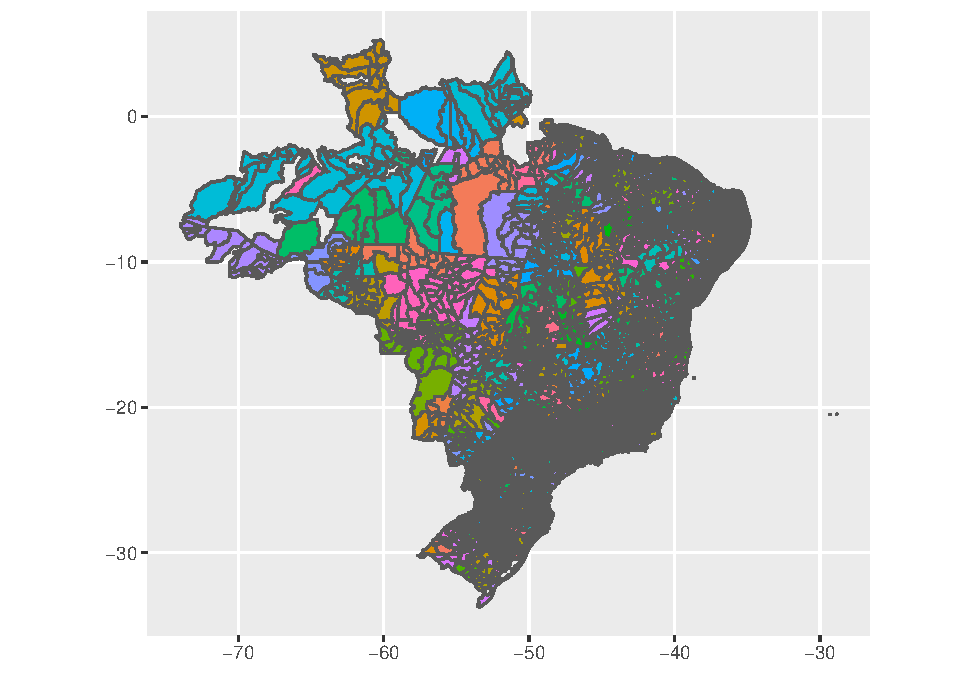
\includegraphics{trabalho_de_conclusao_files/figure-latex/unnamed-chunk-5-1.pdf}

Geramos então. o mapa completo do Brasil divididos por municípios e as
cores representando as áreas atingidas por cada unidade de atendimento,
medido por tempo de viagem de carro, notamos já de início alguns pontos
não categorizados. Como discutido anteriormente, na região norte, com o
parco acesso a infraestrutura rodoviária e grande dependência de viagens
em meio hidroviários, não disponíveis no OpenStreetMap, acaba por não
haver rotas identificadas para estes municípios.

Haveria duas possíveis soluções. Uma solução seria inserir informações
vetoriais de rotas hidrográficas disponíveis na região. A segunda
solução seria a o uso de mapas em grade ( \emph{raster} )
especificamente nessas regiões, para identificas as unidades mais
próximas nos municípios que ficaram de fora. Seja como for, deixa
evidenciado como as diferentes realidades do país impedem a aplicação de
uma única técnicas para todas as situações.

\begin{Shaded}
\begin{Highlighting}[]
\CommentTok{# dados demográficos agregados por unidade de atendimento da RFB }
\NormalTok{aggr <-}\StringTok{ }\NormalTok{map_info }\OperatorTok\StringTok{ }
\StringTok{          }\NormalTok{sf}\OperatorTok{::}\KeywordTok{st_drop_geometry}\NormalTok{() }\OperatorTok\StringTok{ }
\StringTok{          }\KeywordTok{group_by}\NormalTok{(}
\NormalTok{            Unidade, Tipo, Estado, Cidade, Bairro}
\NormalTok{          ) }\OperatorTok\StringTok{ }
\StringTok{          }\KeywordTok{summarise}\NormalTok{(}
\NormalTok{            duraçã}\DataTypeTok{o =} \KeywordTok{mean}\NormalTok{(duração, }\DataTypeTok{na.rm=}\NormalTok{T),}
            \DataTypeTok{salMin_01to02 =} \KeywordTok{sum}\NormalTok{(salMin_01to02, }\DataTypeTok{na.rm =}\NormalTok{ T),}
            \DataTypeTok{salMin_02to05 =} \KeywordTok{sum}\NormalTok{(salMin_02to05, }\DataTypeTok{na.rm =}\NormalTok{ T),}
            \DataTypeTok{salMin_05to10 =} \KeywordTok{sum}\NormalTok{(salMin_05to10, }\DataTypeTok{na.rm =}\NormalTok{ T),}
            \DataTypeTok{salMin_10to20 =} \KeywordTok{sum}\NormalTok{(salMin_10to20, }\DataTypeTok{na.rm =}\NormalTok{ T),}
            \DataTypeTok{salMin_20plus =} \KeywordTok{sum}\NormalTok{(salMin_20plus, }\DataTypeTok{na.rm =}\NormalTok{ T),}
            \DataTypeTok{salMin_semrendimento =} \KeywordTok{sum}\NormalTok{(salMin_semrendimento, }\DataTypeTok{na.rm =}\NormalTok{ T),}
            \DataTypeTok{ativo_2024 =} \KeywordTok{sum}\NormalTok{(ativo_}\DecValTok{2024}\NormalTok{, }\DataTypeTok{na.rm =}\NormalTok{ T),}
            \DataTypeTok{ativo_2529 =} \KeywordTok{sum}\NormalTok{(ativo_}\DecValTok{2529}\NormalTok{, }\DataTypeTok{na.rm =}\NormalTok{ T),}
            \DataTypeTok{ativo_3034 =} \KeywordTok{sum}\NormalTok{(ativo_}\DecValTok{3034}\NormalTok{, }\DataTypeTok{na.rm =}\NormalTok{ T),          }
            \DataTypeTok{ativo_3539 =} \KeywordTok{sum}\NormalTok{(ativo_}\DecValTok{3539}\NormalTok{, }\DataTypeTok{na.rm =}\NormalTok{ T),}
            \DataTypeTok{ativo_4044 =} \KeywordTok{sum}\NormalTok{(ativo_}\DecValTok{4044}\NormalTok{, }\DataTypeTok{na.rm =}\NormalTok{ T),}
            \DataTypeTok{ativo_4549 =} \KeywordTok{sum}\NormalTok{(ativo_}\DecValTok{4549}\NormalTok{, }\DataTypeTok{na.rm =}\NormalTok{ T),}
            \DataTypeTok{ativo_5054 =} \KeywordTok{sum}\NormalTok{(ativo_}\DecValTok{5054}\NormalTok{, }\DataTypeTok{na.rm =}\NormalTok{ T),}
            \DataTypeTok{ativo_5559 =} \KeywordTok{sum}\NormalTok{(ativo_}\DecValTok{5559}\NormalTok{, }\DataTypeTok{na.rm =}\NormalTok{ T),}
            \DataTypeTok{ativo_6069 =} \KeywordTok{sum}\NormalTok{(ativo_}\DecValTok{6069}\NormalTok{, }\DataTypeTok{na.rm =}\NormalTok{ T),          }
            \DataTypeTok{ativo_70plus =} \KeywordTok{sum}\NormalTok{(ativo_70plus, }\DataTypeTok{na.rm =}\NormalTok{ T),}
            \DataTypeTok{ativo_19less =} \KeywordTok{sum}\NormalTok{(ativo_19less, }\DataTypeTok{na.rm =}\NormalTok{ T),}
            \DataTypeTok{inativo_2024 =} \KeywordTok{sum}\NormalTok{(inativo_}\DecValTok{2024}\NormalTok{, }\DataTypeTok{na.rm =}\NormalTok{ T),}
            \DataTypeTok{inativo_2529 =} \KeywordTok{sum}\NormalTok{(inativo_}\DecValTok{2529}\NormalTok{, }\DataTypeTok{na.rm =}\NormalTok{ T),}
            \DataTypeTok{inativo_3034 =} \KeywordTok{sum}\NormalTok{(inativo_}\DecValTok{3034}\NormalTok{, }\DataTypeTok{na.rm =}\NormalTok{ T),}
            \DataTypeTok{inativo_3539 =} \KeywordTok{sum}\NormalTok{(inativo_}\DecValTok{3539}\NormalTok{, }\DataTypeTok{na.rm =}\NormalTok{ T),}
            \DataTypeTok{inativo_4044 =} \KeywordTok{sum}\NormalTok{(inativo_}\DecValTok{4044}\NormalTok{, }\DataTypeTok{na.rm =}\NormalTok{ T),}
            \DataTypeTok{inativo_4549 =} \KeywordTok{sum}\NormalTok{(inativo_}\DecValTok{4549}\NormalTok{, }\DataTypeTok{na.rm =}\NormalTok{ T),}
            \DataTypeTok{inativo_5054 =} \KeywordTok{sum}\NormalTok{(inativo_}\DecValTok{5054}\NormalTok{, }\DataTypeTok{na.rm =}\NormalTok{ T),}
            \DataTypeTok{inativo_5559 =} \KeywordTok{sum}\NormalTok{(inativo_}\DecValTok{5559}\NormalTok{, }\DataTypeTok{na.rm =}\NormalTok{ T),}
            \DataTypeTok{inativo_6069 =} \KeywordTok{sum}\NormalTok{(inativo_}\DecValTok{6069}\NormalTok{, }\DataTypeTok{na.rm =}\NormalTok{ T),}
            \DataTypeTok{inativo_70plus =} \KeywordTok{sum}\NormalTok{(inativo_70plus, }\DataTypeTok{na.rm =}\NormalTok{ T),}
            \DataTypeTok{inativo_19less =} \KeywordTok{sum}\NormalTok{(inativo_19less, }\DataTypeTok{na.rm =}\NormalTok{ T)}
\NormalTok{          ) }\OperatorTok\StringTok{ }
\StringTok{        }\KeywordTok{ungroup}\NormalTok{()}
\end{Highlighting}
\end{Shaded}

\begin{Shaded}
\begin{Highlighting}[]
\NormalTok{tempoViag <-}\StringTok{ }\KeywordTok{ggplot}\NormalTok{(aggr, }\KeywordTok{aes}\NormalTok{(}\DataTypeTok{x =} \KeywordTok{reorder}\NormalTok{(Unidade, duração), }\DataTypeTok{y=}\NormalTok{ duração)) }\OperatorTok{+}\StringTok{ }\KeywordTok{geom_bar}\NormalTok{(}\DataTypeTok{stat =} \StringTok{'identity'}\NormalTok{) }\OperatorTok{+}\StringTok{ }\KeywordTok{theme_minimal}\NormalTok{() }\OperatorTok{+}\StringTok{ }\KeywordTok{theme}\NormalTok{(}\DataTypeTok{axis.text.x =} \KeywordTok{element_blank}\NormalTok{())}
\NormalTok{tempoViag}
\end{Highlighting}
\end{Shaded}

\includegraphics{trabalho_de_conclusao_files/figure-latex/unnamed-chunk-7-1.pdf}

Ao analisarmos o tempo de viagem entre os municípios e suas respectivas
unidades de atendimento, percebemos que há uma grande uniformidade, mas
com alguns outliers com tempos fora do normal.

\begin{Shaded}
\begin{Highlighting}[]
\KeywordTok{summary}\NormalTok{(aggr}\OperatorTok{$}\NormalTok{duração)}
\end{Highlighting}
\end{Shaded}

\begin{verbatim}
##    Min. 1st Qu.  Median    Mean 3rd Qu.    Max. 
##    0.00   28.34   42.67   76.16   65.62 7944.81
\end{verbatim}

Em verdade, percebemos que o tempo mediano de viagem para uma unidade de
atendimento é de 42 minutos de carro, e a média vai para 76 minutos,
certamente puxado pelos outliers.

\begin{Shaded}
\begin{Highlighting}[]
\NormalTok{pop_outlier <-}\StringTok{ }\NormalTok{aggr }\OperatorTok\StringTok{ }\KeywordTok{filter}\NormalTok{(duração }\OperatorTok{>}\StringTok{ }\KeywordTok{mean}\NormalTok{(aggr}\OperatorTok{$}\NormalTok{duração)) }\OperatorTok\StringTok{ }\KeywordTok{select}\NormalTok{(ativo_}\DecValTok{2024}\OperatorTok{:}\NormalTok{inativo_19less) }\OperatorTok\StringTok{ }\KeywordTok{mutate}\NormalTok{(}\DataTypeTok{total =} \KeywordTok{rowSums}\NormalTok{(., }\DataTypeTok{na.rm =}\NormalTok{ T))}
\KeywordTok{sum}\NormalTok{(pop_outlier}\OperatorTok{$}\NormalTok{total)}
\end{Highlighting}
\end{Shaded}

\begin{verbatim}
## [1] 33478112
\end{verbatim}

É possível que esses outliers existam pelas já discutidas limitações na
infraestrutura rodoviária, mas seria interessante analisar com mais
calma a situação dos municípios que estão muito acima da média, de um
ponto de vista de garantia da acessibilidade. Afinal, como podemos ver
acima, são 3 milhões e 300 mil pessoas nessa situação.

\begin{Shaded}
\begin{Highlighting}[]
\NormalTok{popUnidades <-}\StringTok{ }\NormalTok{aggr }\OperatorTok\StringTok{ }\KeywordTok{select}\NormalTok{(Unidade, ativo_}\DecValTok{2024}\OperatorTok{:}\NormalTok{inativo_19less) }\OperatorTok\StringTok{ }\KeywordTok{mutate}\NormalTok{(}\DataTypeTok{total =} \KeywordTok{rowSums}\NormalTok{(.[}\DecValTok{2}\OperatorTok{:}\KeywordTok{ncol}\NormalTok{(.)], }\DataTypeTok{na.rm =}\NormalTok{ T))}
\NormalTok{popUnidsChart <-}\StringTok{ }\KeywordTok{ggplot}\NormalTok{(popUnidades, }\KeywordTok{aes}\NormalTok{(}\DataTypeTok{x =} \KeywordTok{reorder}\NormalTok{(Unidade, total), }\DataTypeTok{y=}\NormalTok{ total))}\OperatorTok{+}\StringTok{ }\KeywordTok{geom_bar}\NormalTok{(}\DataTypeTok{stat =} \StringTok{'identity'}\NormalTok{) }\OperatorTok{+}\StringTok{ }\KeywordTok{theme_minimal}\NormalTok{() }\OperatorTok{+}\StringTok{ }\KeywordTok{theme}\NormalTok{(}\DataTypeTok{axis.text.x =} \KeywordTok{element_blank}\NormalTok{())}
\NormalTok{popUnidsChart}
\end{Highlighting}
\end{Shaded}

\includegraphics{trabalho_de_conclusao_files/figure-latex/unnamed-chunk-10-1.pdf}

\begin{Shaded}
\begin{Highlighting}[]
\KeywordTok{summary}\NormalTok{(popUnidades}\OperatorTok{$}\NormalTok{total)}
\end{Highlighting}
\end{Shaded}

\begin{verbatim}
##      Min.   1st Qu.    Median      Mean   3rd Qu.      Max. 
##     19577    164968    262686    867280    398886 120726288
\end{verbatim}

Ao levantarmos a população total atingida, novamente encontramos cenário
de grandes desigualdades, que mereceriam atenção para um planejamento
mais estratégico do posicionamento das unidades. A média de pessoas
dentro do público-alvo das unidades é de cerca de 870 mil, mas essa
média é fortemente puxada por outliers com um número muito alto de
atingidos. A unidade com maior número de atendidos chega a uma população
estimada de 12 milhões de pessoas, enquanto a menor unidade atinge
apenas 20 mil pessoa.

Entretanto, até o momento, estamos tratando a população inteira dos
municípios como população-alvo das unidades de atendimento. Na prática,
aqueles que não possuem renda, que estejam economicamente inativos, em
geral, não possuem grandes motivos para lidar com a Receita Federal.
Ademais, há também o argumento de que o serviços presenciais servem
principalmente às populações mais velhas, com menos familiaridade com os
canais digitais. Essas seleções são exemplos de como se poderia refinar
e definir com mais precisão o público das unidades de atendimento, a fim
de prestar um melhor serviço.

Primeiramente, podemos analisar a idade média da população
econômicamente ativa atendida por cada unidade.

\begin{Shaded}
\begin{Highlighting}[]
\NormalTok{meanAge <-}\StringTok{ }\NormalTok{aggr }\OperatorTok\StringTok{ }
\StringTok{              }\KeywordTok{select}\NormalTok{(Unidade, ativo_}\DecValTok{2024}\OperatorTok{:}\NormalTok{ativo_19less) }\OperatorTok\StringTok{ }
\StringTok{              }\KeywordTok{mutate}\NormalTok{(}
                \DataTypeTok{total =} \KeywordTok{rowSums}\NormalTok{(.[}\DecValTok{2}\OperatorTok{:}\KeywordTok{ncol}\NormalTok{(.)]),}
                
                \DataTypeTok{weightAge =}\NormalTok{ (ativo_}\DecValTok{2024} \OperatorTok{*}\StringTok{ }\NormalTok{(}\DecValTok{20}\OperatorTok{+}\DecValTok{24}\NormalTok{)}\OperatorTok{/}\DecValTok{2} \OperatorTok{+}
\StringTok{                }\NormalTok{ativo_}\DecValTok{2529} \OperatorTok{*}\StringTok{ }\NormalTok{(}\DecValTok{25}\OperatorTok{+}\DecValTok{29}\NormalTok{)}\OperatorTok{/}\DecValTok{2} \OperatorTok{+}\StringTok{ }
\StringTok{                }\NormalTok{ativo_}\DecValTok{3034} \OperatorTok{*}\StringTok{ }\NormalTok{(}\DecValTok{30}\OperatorTok{+}\DecValTok{34}\NormalTok{)}\OperatorTok{/}\DecValTok{2} \OperatorTok{+}
\StringTok{                }\NormalTok{ativo_}\DecValTok{3539} \OperatorTok{*}\StringTok{ }\NormalTok{(}\DecValTok{35}\OperatorTok{+}\DecValTok{39}\NormalTok{)}\OperatorTok{/}\DecValTok{2} \OperatorTok{+}
\StringTok{                }\NormalTok{ativo_}\DecValTok{4044} \OperatorTok{*}\StringTok{ }\NormalTok{(}\DecValTok{40}\OperatorTok{+}\DecValTok{44}\NormalTok{)}\OperatorTok{/}\DecValTok{2} \OperatorTok{+}
\StringTok{                }\NormalTok{ativo_}\DecValTok{4549} \OperatorTok{*}\StringTok{ }\NormalTok{(}\DecValTok{45}\OperatorTok{+}\DecValTok{49}\NormalTok{)}\OperatorTok{/}\DecValTok{2} \OperatorTok{+}
\StringTok{                }\NormalTok{ativo_}\DecValTok{5054} \OperatorTok{*}\StringTok{ }\NormalTok{(}\DecValTok{50}\OperatorTok{+}\DecValTok{54}\NormalTok{)}\OperatorTok{/}\DecValTok{2} \OperatorTok{+}
\StringTok{                }\NormalTok{ativo_}\DecValTok{5559} \OperatorTok{*}\StringTok{ }\NormalTok{(}\DecValTok{55}\OperatorTok{+}\DecValTok{59}\NormalTok{)}\OperatorTok{/}\DecValTok{2} \OperatorTok{+}
\StringTok{                }\NormalTok{ativo_}\DecValTok{6069} \OperatorTok{*}\StringTok{ }\NormalTok{(}\DecValTok{60}\OperatorTok{+}\DecValTok{69}\NormalTok{)}\OperatorTok{/}\DecValTok{2} \OperatorTok{+}
\StringTok{                }\NormalTok{ativo_70plus }\OperatorTok{*}\StringTok{ }\NormalTok{(}\DecValTok{70}\OperatorTok{+}\DecValTok{100}\NormalTok{)}\OperatorTok{/}\DecValTok{2} \OperatorTok{+}
\StringTok{                }\NormalTok{ativo_19less }\OperatorTok{*}\StringTok{ }\NormalTok{(}\DecValTok{19}\NormalTok{)}\OperatorTok{/}\DecValTok{2}\NormalTok{) }\OperatorTok{/}\StringTok{ }\NormalTok{total}
\NormalTok{              ) }\OperatorTok\StringTok{ }
\StringTok{              }\KeywordTok{filter}\NormalTok{(weightAge }\OperatorTok{<=}\StringTok{ }\KeywordTok{max}\NormalTok{(weightAge))}


\NormalTok{meanAgeChart <-}\StringTok{ }\KeywordTok{ggplot}\NormalTok{(meanAge, }\KeywordTok{aes}\NormalTok{(}\DataTypeTok{x =} \KeywordTok{reorder}\NormalTok{(Unidade, weightAge), }\DataTypeTok{y =}\NormalTok{ weightAge)) }\OperatorTok{+}\StringTok{ }\KeywordTok{geom_point}\NormalTok{()}\OperatorTok{+}\StringTok{  }\KeywordTok{theme}\NormalTok{(}\DataTypeTok{axis.text.x =} \KeywordTok{element_blank}\NormalTok{())}
\NormalTok{meanAgeChart}
\end{Highlighting}
\end{Shaded}

\includegraphics{trabalho_de_conclusao_files/figure-latex/unnamed-chunk-12-1.pdf}

A idade média das unidades de atendimento aponta para uma população
economicamente ativa relativamente jovem, com idade média próxima dos 36
anos de idade. Todavia, não podemos nos esquecer que estes dados são do
censo de 2010, e o próximo censo, de 2020, pode já apontar uma população
mais envelhecida.

\begin{Shaded}
\begin{Highlighting}[]
\KeywordTok{summary}\NormalTok{(meanAge}\OperatorTok{$}\NormalTok{weightAge)}
\end{Highlighting}
\end{Shaded}

\begin{verbatim}
##    Min. 1st Qu.  Median    Mean 3rd Qu.    Max. 
##   33.40   36.00   36.79   36.83   37.58   41.93
\end{verbatim}

\begin{Shaded}
\begin{Highlighting}[]
\NormalTok{meanAgeTodos <-}\StringTok{ }\NormalTok{aggr }\OperatorTok\StringTok{ }
\StringTok{              }\KeywordTok{select}\NormalTok{(Unidade, ativo_}\DecValTok{2024}\OperatorTok{:}\NormalTok{inativo_19less) }\OperatorTok\StringTok{ }
\StringTok{              }\KeywordTok{mutate}\NormalTok{(}
                \DataTypeTok{total =} \KeywordTok{rowSums}\NormalTok{(.[}\DecValTok{2}\OperatorTok{:}\KeywordTok{ncol}\NormalTok{(.)]),}
                
                \DataTypeTok{weightAge =}\NormalTok{ (ativo_}\DecValTok{2024} \OperatorTok{*}\StringTok{ }\NormalTok{(}\DecValTok{20}\OperatorTok{+}\DecValTok{24}\NormalTok{)}\OperatorTok{/}\DecValTok{2} \OperatorTok{+}
\StringTok{                }\NormalTok{ativo_}\DecValTok{2529} \OperatorTok{*}\StringTok{ }\NormalTok{(}\DecValTok{25}\OperatorTok{+}\DecValTok{29}\NormalTok{)}\OperatorTok{/}\DecValTok{2} \OperatorTok{+}\StringTok{ }
\StringTok{                }\NormalTok{ativo_}\DecValTok{3034} \OperatorTok{*}\StringTok{ }\NormalTok{(}\DecValTok{30}\OperatorTok{+}\DecValTok{34}\NormalTok{)}\OperatorTok{/}\DecValTok{2} \OperatorTok{+}
\StringTok{                }\NormalTok{ativo_}\DecValTok{3539} \OperatorTok{*}\StringTok{ }\NormalTok{(}\DecValTok{35}\OperatorTok{+}\DecValTok{39}\NormalTok{)}\OperatorTok{/}\DecValTok{2} \OperatorTok{+}
\StringTok{                }\NormalTok{ativo_}\DecValTok{4044} \OperatorTok{*}\StringTok{ }\NormalTok{(}\DecValTok{40}\OperatorTok{+}\DecValTok{44}\NormalTok{)}\OperatorTok{/}\DecValTok{2} \OperatorTok{+}
\StringTok{                }\NormalTok{ativo_}\DecValTok{4549} \OperatorTok{*}\StringTok{ }\NormalTok{(}\DecValTok{45}\OperatorTok{+}\DecValTok{49}\NormalTok{)}\OperatorTok{/}\DecValTok{2} \OperatorTok{+}
\StringTok{                }\NormalTok{ativo_}\DecValTok{5054} \OperatorTok{*}\StringTok{ }\NormalTok{(}\DecValTok{50}\OperatorTok{+}\DecValTok{54}\NormalTok{)}\OperatorTok{/}\DecValTok{2} \OperatorTok{+}
\StringTok{                }\NormalTok{ativo_}\DecValTok{5559} \OperatorTok{*}\StringTok{ }\NormalTok{(}\DecValTok{55}\OperatorTok{+}\DecValTok{59}\NormalTok{)}\OperatorTok{/}\DecValTok{2} \OperatorTok{+}
\StringTok{                }\NormalTok{ativo_}\DecValTok{6069} \OperatorTok{*}\StringTok{ }\NormalTok{(}\DecValTok{60}\OperatorTok{+}\DecValTok{69}\NormalTok{)}\OperatorTok{/}\DecValTok{2} \OperatorTok{+}
\StringTok{                }\NormalTok{ativo_70plus }\OperatorTok{*}\StringTok{ }\NormalTok{(}\DecValTok{70}\OperatorTok{+}\DecValTok{100}\NormalTok{)}\OperatorTok{/}\DecValTok{2} \OperatorTok{+}
\StringTok{                }\NormalTok{ativo_19less }\OperatorTok{*}\StringTok{ }\NormalTok{(}\DecValTok{19}\NormalTok{)}\OperatorTok{/}\DecValTok{2} \OperatorTok{+}
\StringTok{                  }
\StringTok{                }\NormalTok{inativo_}\DecValTok{2024} \OperatorTok{*}\StringTok{ }\NormalTok{(}\DecValTok{20}\OperatorTok{+}\DecValTok{24}\NormalTok{)}\OperatorTok{/}\DecValTok{2} \OperatorTok{+}
\StringTok{                }\NormalTok{inativo_}\DecValTok{2529} \OperatorTok{*}\StringTok{ }\NormalTok{(}\DecValTok{25}\OperatorTok{+}\DecValTok{29}\NormalTok{)}\OperatorTok{/}\DecValTok{2} \OperatorTok{+}\StringTok{ }
\StringTok{                }\NormalTok{inativo_}\DecValTok{3034} \OperatorTok{*}\StringTok{ }\NormalTok{(}\DecValTok{30}\OperatorTok{+}\DecValTok{34}\NormalTok{)}\OperatorTok{/}\DecValTok{2} \OperatorTok{+}
\StringTok{                }\NormalTok{inativo_}\DecValTok{3539} \OperatorTok{*}\StringTok{ }\NormalTok{(}\DecValTok{35}\OperatorTok{+}\DecValTok{39}\NormalTok{)}\OperatorTok{/}\DecValTok{2} \OperatorTok{+}
\StringTok{                }\NormalTok{inativo_}\DecValTok{4044} \OperatorTok{*}\StringTok{ }\NormalTok{(}\DecValTok{40}\OperatorTok{+}\DecValTok{44}\NormalTok{)}\OperatorTok{/}\DecValTok{2} \OperatorTok{+}
\StringTok{                }\NormalTok{inativo_}\DecValTok{4549} \OperatorTok{*}\StringTok{ }\NormalTok{(}\DecValTok{45}\OperatorTok{+}\DecValTok{49}\NormalTok{)}\OperatorTok{/}\DecValTok{2} \OperatorTok{+}
\StringTok{                }\NormalTok{inativo_}\DecValTok{5054} \OperatorTok{*}\StringTok{ }\NormalTok{(}\DecValTok{50}\OperatorTok{+}\DecValTok{54}\NormalTok{)}\OperatorTok{/}\DecValTok{2} \OperatorTok{+}
\StringTok{                }\NormalTok{inativo_}\DecValTok{5559} \OperatorTok{*}\StringTok{ }\NormalTok{(}\DecValTok{55}\OperatorTok{+}\DecValTok{59}\NormalTok{)}\OperatorTok{/}\DecValTok{2} \OperatorTok{+}
\StringTok{                }\NormalTok{inativo_}\DecValTok{6069} \OperatorTok{*}\StringTok{ }\NormalTok{(}\DecValTok{60}\OperatorTok{+}\DecValTok{69}\NormalTok{)}\OperatorTok{/}\DecValTok{2} \OperatorTok{+}
\StringTok{                }\NormalTok{inativo_70plus }\OperatorTok{*}\StringTok{ }\NormalTok{(}\DecValTok{70}\OperatorTok{+}\DecValTok{100}\NormalTok{)}\OperatorTok{/}\DecValTok{2} \OperatorTok{+}
\StringTok{                }\NormalTok{inativo_19less }\OperatorTok{*}\StringTok{ }\NormalTok{(}\DecValTok{19}\NormalTok{)}\OperatorTok{/}\DecValTok{2}
                  
\NormalTok{                ) }\OperatorTok{/}\StringTok{ }\NormalTok{total}
\NormalTok{              ) }\OperatorTok\StringTok{ }
\StringTok{              }\KeywordTok{filter}\NormalTok{(weightAge }\OperatorTok{<=}\StringTok{ }\KeywordTok{max}\NormalTok{(weightAge))}

\KeywordTok{summary}\NormalTok{(meanAgeTodos}\OperatorTok{$}\NormalTok{weightAge)}
\end{Highlighting}
\end{Shaded}

\begin{verbatim}
##    Min. 1st Qu.  Median    Mean 3rd Qu.    Max. 
##   29.37   34.41   35.73   35.64   37.02   44.47
\end{verbatim}

Mesmo quando incluímos os inativos, as médias e medianas permanecem em
torno de 35 anos, indicando-nos que as unidades atendem uma população
mais jovem, que provavelmente possui mais contato e conhecimento de uso
dos canais digitais.

Em verdade, se formos investigar o percentual de pessoas com mais de 60
anos de idade, percebemos que eles não representam uma parcela relevante
para praticamente nenhuma das unidades.

\begin{Shaded}
\begin{Highlighting}[]
\NormalTok{pop60plus <-}\StringTok{ }\NormalTok{aggr }\OperatorTok\StringTok{ }
\StringTok{                    }\KeywordTok{select}\NormalTok{(Unidade, ativo_}\DecValTok{2024}\OperatorTok{:}\NormalTok{inativo_19less) }\OperatorTok\StringTok{ }
\StringTok{                    }\KeywordTok{mutate}\NormalTok{(}
                      \DataTypeTok{total =} \KeywordTok{rowSums}\NormalTok{(.[}\DecValTok{2}\OperatorTok{:}\KeywordTok{ncol}\NormalTok{(.)], }\DataTypeTok{na.rm=}\NormalTok{T),}
                      \DataTypeTok{perc_60plus =}\NormalTok{ (ativo_}\DecValTok{6069}\OperatorTok{+}\NormalTok{ativo_70plus}\OperatorTok{+}\NormalTok{inativo_}\DecValTok{6069}\OperatorTok{+}\NormalTok{inativo_70plus)}\OperatorTok{/}\NormalTok{total}
\NormalTok{                    )}
\NormalTok{plu60Chart <-}\StringTok{ }\KeywordTok{ggplot}\NormalTok{(pop60plus, }\KeywordTok{aes}\NormalTok{(}\DataTypeTok{x =} \KeywordTok{reorder}\NormalTok{(Unidade, perc_60plus), }\DataTypeTok{y =}\NormalTok{ perc_60plus)) }\OperatorTok{+}\StringTok{ }\KeywordTok{geom_point}\NormalTok{()}\OperatorTok{+}\StringTok{  }\KeywordTok{theme}\NormalTok{(}\DataTypeTok{axis.text.x =} \KeywordTok{element_blank}\NormalTok{())}
\NormalTok{plu60Chart}
\end{Highlighting}
\end{Shaded}

\includegraphics{trabalho_de_conclusao_files/figure-latex/unnamed-chunk-15-1.pdf}

\begin{Shaded}
\begin{Highlighting}[]
\KeywordTok{summary}\NormalTok{(pop60plus}\OperatorTok{$}\NormalTok{perc_60plus)}
\end{Highlighting}
\end{Shaded}

\begin{verbatim}
##    Min. 1st Qu.  Median    Mean 3rd Qu.    Max. 
## 0.05517 0.11543 0.13128 0.13130 0.14802 0.23851
\end{verbatim}

Em termos percentuais, estamos falando de no máximo 23\% da população,
mas a média e a mediana estão firmes em torno de 13\%, portanto, em
média, 87\% da população encontra-se abaixo dessa faixa etária.

Uma última análise interessante seria em relação à renda. Independente
da idade, os principais motivos para que pessoas físicas se dirijam a
unidades de atendimento da Receita Federal são o Cadastro de Pessoas
Física (CPF) e a DIRPF (Declaração de Imposto de Renda de Pessoa
Física). O CPF pode ser gerado, alterado e cancelado em diversos outros
órgãos conveniados, incluindo os Correios e o Banco do Brasil. o que
diminuir fortemente a necessidade do cidadão se deslocar a um posto de
atendimento da RFB. A DIRPF, por outro lado, só pode ser resolvida na
própria instituição.

Assim, podemos argumentar que o público-alvo, neste caso, se
restringiria apenas àqueles que tivessem renda mensal acima de 4
salários mínimos, posto que o salário mínimo correspondia a R\$ 510,00
em 2010, ano do Censo. Como não temos o quantitativo de pessoas que
ganham entre 4 e 5 salários mínimos separado, podemos analisar qual o
percentual e o número absoluto da população que ganha acima de 5
salários mínimos, de acordo com o censo de 2010, como uma aproximação do
que queremos visualizar.

\begin{Shaded}
\begin{Highlighting}[]
\NormalTok{popIrpf <-}\StringTok{ }\NormalTok{aggr }\OperatorTok\StringTok{ }
\StringTok{                    }\KeywordTok{select}\NormalTok{(Unidade, salMin_01to02}\OperatorTok{:}\NormalTok{salMin_semrendimento) }\OperatorTok\StringTok{ }
\StringTok{                    }\KeywordTok{mutate}\NormalTok{(}
                      \DataTypeTok{total =} \KeywordTok{rowSums}\NormalTok{(.[}\DecValTok{2}\OperatorTok{:}\KeywordTok{ncol}\NormalTok{(.)], }\DataTypeTok{na.rm=}\NormalTok{T),}
                      \DataTypeTok{perc_more05 =} \DecValTok{1}\OperatorTok{-}\NormalTok{((salMin_01to02}\OperatorTok{+}\NormalTok{salMin_semrendimento}\OperatorTok{+}\NormalTok{salMin_02to05)}\OperatorTok{/}\NormalTok{total)}
\NormalTok{                    )}

\NormalTok{popIrpfChart <-}\StringTok{ }\KeywordTok{ggplot}\NormalTok{(popIrpf, }\KeywordTok{aes}\NormalTok{(}\DataTypeTok{x =} \KeywordTok{reorder}\NormalTok{(Unidade, perc_more05), }\DataTypeTok{y =}\NormalTok{ perc_more05)) }\OperatorTok{+}\StringTok{ }\KeywordTok{geom_point}\NormalTok{()}\OperatorTok{+}\StringTok{  }\KeywordTok{theme}\NormalTok{(}\DataTypeTok{axis.text.x =} \KeywordTok{element_blank}\NormalTok{())}
\NormalTok{popIrpfChart}
\end{Highlighting}
\end{Shaded}

\includegraphics{trabalho_de_conclusao_files/figure-latex/unnamed-chunk-17-1.pdf}

\begin{Shaded}
\begin{Highlighting}[]
\KeywordTok{summary}\NormalTok{(popIrpf}\OperatorTok{$}\NormalTok{perc_more05)}
\end{Highlighting}
\end{Shaded}

\begin{verbatim}
##    Min. 1st Qu.  Median    Mean 3rd Qu.    Max. 
## 0.04292 0.08581 0.09942 0.11252 0.12014 0.45919
\end{verbatim}

A informação que tiramos é que a população brasileira é bastante
carente, e que a parcela que tem mais contato com a Receita Federal é
bastante pequena. Enquanto há unidades atendendo a um máximo de 46\% do
público-alvo, a média e a mediana são em torno de 10\%, com um mínimo de
4\% do público-alvo. Todas essas análises são aproximações, utilizando
dados antigos, do Censo de 2010. Todavia, podem ser refinados, e mesmo
como aproximações, já nos servem para algumas lições.

Percebemos que a população atingida por cada uma das unidades da Receita
Federal é, no geral, relativamente pobre e relativamente jovem. Disso,
tiramos que, por um lado, é uma população que não deveria ter grande
dificuldade de aprender a acessar os canais digitais, para os que
necessitassem de acesso, o que, pela análise da renda, não é uma parcela
tão grande da população.

Por outro lado, a Receita Federal poderia desde já, buscar aumentar o
foco de suas unidades presenciais. Estudar os pontos fora da curva de
população atingida e de duração de viagem poderiam das \emph{insights}
importantes sobre possíveis fechamentos e aberturas de unidades,
reorganizando a distribuição no território da população e buscando
aumentar a acessibilidade de seus serviços.

Acima de tudo, nos ensina que há ineficiências que podem ser
visualizadas com a mais simples das aproximações analíticas, e que,
portanto, existe um potencial significativo no uso de análise de dados
para a gestão do atendimento da Receita Federal do Brasil.

\hypertarget{atendimento-tributario-como-politica-publica}{%
\subsection{3.3 Atendimento tributário como política
pública}\label{atendimento-tributario-como-politica-publica}}

Políticas públicas são respostas intencionais do Estado a um problema
específico, seja pela ação ou pela omissão. Como tal, são definidas em
torno de um problema enfrentado por uma seção da população. Para serem
efetivas, as políticas públicas devem ser construídas de forma a
maximizar o efeito dos recursos empregados sobre a população-alvo ao
mesmo tempo em que se minimiza o dispêndio de recursos com aqueles fora
da população-alvo, de forma a garantir a eficiência da resposta do
Estado.

A definição de qual é a população-alvo de uma política pública, é
portanto, um dos pontos mais cruciais para garantir sua eficiência,
eficácia e efetividade. Se essa população não estiver bem definida,
corre-se o risco de, dentro de um orçamento finito, não haver recursos o
suficiente para resolver o problema para o qual a política pública foi
inicialmente desenhada.

A disponibilização de atendimento presencial na Receita Federal do
Brasil é uma política pública. O serviço serve, primordialmente, para
garantir que o cidadão terá acesso não só a informações necessárias para
agir em conformidade com a norma tributária, mas também e eventualmente,
ter acesso aos meios de efetivar essa conformidade, pela entrega e
emissão de documentos e formulários assim como na geração e atualização
de cadastros e outras informações.

Com o avanço da digitalização dos serviços governamentais, cabe ao
Estado repensar o público-alvo do atendimento presencial. Como o custo
do atendimento digital é múltiplas vezes menor que o de manter postos de
atendimento presenciais, cabe ao Estado equilibrar a garantia de acesso
com a disponibilidade de recursos, buscando um ponto que maximize as
duas variáveis conflitantes. Este ponto de equilíbrio muito
provavelmente estará na oferta do serviço presencial preferencialmente
àqueles que não podem ou não saber como acessar digitalmente.O primeiro
passo, portanto, é identificar, hoje, quem são essas pessoas.

Seria interessante que a Receita Federal do Brasil testasse hipóteses em
cima das relações entre variáveis demográficas como renda, idade, gênero
e nível educacional e a preferência entre os canais digitais e
presenciais. Esses estudos podem ser realizados em cima das bases de
dado internas de acesso ao e-Cac e de atendimentos realizados, estes
últimos registrados no Sistema Nacional de Apoio ao Gerenciamento de
Atendimento (SAGA).

O SAGA, ou Sistema Nacional de Apoio ao Gerenciamento do Atendimento, é
um sistema eletrônico de coleta de dados e gerenciamento do atendimento
da Receita Federal, em todas as suas etapas. Como tal, é o sistema que
melhor permitiria à instituição conhecer o perfil demográfico de seu
público-alvo, e, cruzando com dados do IBGE e de outras fontes, medir o
nível de acesso de cada setor da população aos serviços presenciais da
secretaria.

Para avaliarmos esse nível de acesso, poderia-se expandir o processo de
mensuração do acesso realizado nesse artigo. Uma primeira opção seria
realizar comparação mais paciente entre o uso de mapas de grade e mapas
de rede, especialmente nas regiões do país com menor acesso à
infraestrutura de transporte. A comparação forneceria maior
flexibilidade ao modelo, buscando-se a melhor simulação possível.

Segunda opção seria, em vez de utilizar apenas os dados do
OpenStreetMap, adicionar mais bases de dados de infraestrutura e mais
modais de transporte, como o hidroviário no norte do país. Aumentaria-se
assim o realismo do modelo geográfico, possibilitando a construção de
estimativas mais úteis.

Por fim, devemos entender que isso é um processo, não um projeto, ou
seja, ele é contínuo no tempo. À medida que os canais de atendimento
presencial e físico vão se modificando, e a população também se
modifica, novos testes devem ser realizados continuamente, seguindo o
tradicional ciclo de planejamento, execução, controle e avaliação.
Métricas devem ser estabelecidas e melhorias implementadas, buscando
fidedignidade no modelo.

Acreditamos que, dessa forma, estará estabelecido um processo de
planejamento do atendimento presencial com foco no cidadão, otimizando o
gasto público mas sem deixar de lado a garantia do direito de acesso
desse ao serviço público.

\hypertarget{conclusao}{%
\section{Conclusão}\label{conclusao}}

Neste artigo, sugeririmos um processo baseado em dados para distribuir
as unidades de atendimento presencial da Receita Federal do Brasil. Da
análise que realizamos sobre o público-alvo teórico das unidades atuais,
percebemos que a quantidade de pessoas teoricamente atingidas, quando
selecionadas por renda e/ou idade, é uma parcela relativamente pequena
da população. Ademais, outliers na distribuição do total de atingidos e
na distância em tempo de viagem nos sugere que há ineficiências a serem
sanadas, por um lado populações desasistidas, longe demais das unidades
presentes, por outro lado, unidades que atingem população ínfima, de
necessidade duvidosa.

Várias são as avenidas para aplicarmos os modelos deste artigo na
prática. Primeiro, poderíamos melhorarm os dados geográficos atuais,
inserindo informações de outros meios de transporte como o hidroviário,
largamente utilizado na região Norte. Segundo, poderíamos atualizar os
dados demográficos, não só com os resultados do iminente Censo 2020, mas
também com outras fontes de informações. Terceiro, poderíamos cruzar
essas informações com dados reais dos atendimentos realizados,
permitindo-nos estimar os fatores mais relevantes para a escolha da
unidade de atendimento por um contribuinte.

Com tudo isso, afirmamos ter demonstrado a plena viabilidade de se tomar
decisões quanto a estratégia de atendimento da Receita Federal do Brasil
de forma imparcial, objetiva, e com o foco no melhor atendimento ao
cidadão que efetivamente utiliza seus serviços.

\hypertarget{referencias}{%
\subsection*{Referências}\label{referencias}}
\addcontentsline{toc}{subsection}{Referências}

\hypertarget{refs}{}
\leavevmode\hypertarget{ref-tribunal_de_contas_da_uniao_auditoria_2017}{}%
Contas da União, Tribunal de. 2017. ``Auditoria Operacional Realizada Na
Secretaria Da Receita Federal Do Brasil.''

\leavevmode\hypertarget{ref-delamater_measuring_2012}{}%
Delamater, Paul, Joseph Messina, Ashton M Shortridge, and Sue C Grady.
2012. ``Measuring Geographic Access to Health Care: Raster and
Network-Based Methods.'' \emph{International Journal of Health
Geographics} 11 (May): 15.
\url{https://doi.org/10.1186/1476-072X-11-15}.

\leavevmode\hypertarget{ref-j._weiss_global_2018}{}%
J. Weiss, D, Andy Nelson, Harry Gibson, W Temperley, Stephen Peedel, A
Lieber, M Hancher, et al. 2018. ``A Global Map of Travel Time to Cities
to Assess Inequalities in Accessibility in 2015.'' \emph{Nature} 553
(7688).
\url{https://www.researchgate.net/publication/322368535_A_global_map_of_travel_time_to_cities_to_assess_inequalities_in_accessibility_in_2015?_sg=Im7RuSiWTkiNinanqup8V53CG0MB12I6dJ_p_Dvci_6XlpcaXrK517NFRuTIudP0Temj5nV3IkWmaog}.

\leavevmode\hypertarget{ref-noor_defining_2003}{}%
Noor, Abdisalan, Simon Iain Hay, D Zurovac, S.A. Ochola, and Robert W
Snow. 2003. ``Defining Equity in Physical Access to Clinical Services
Using Geographical Information Systems as Part of Malaria Planning and
Monitoring in Kenya.'' \emph{Tropical Medicine \& International Health}
8 (10): 917--26.
\url{https://www.researchgate.net/publication/9075228_Defining_Equity_in_Physical_Access_to_Clinical_Services_Using_Geographical_Information_Systems_as_Part_of_Malaria_Planning_and_Monitoring_in_Kenya}.

\leavevmode\hypertarget{ref-thaddeus_too_1994}{}%
Thaddeus, Sereen, and Deborah Maine. 1994. ``Too Far to Walk: Maternal
Mortality in Context.'' \emph{Social Science \& Medicine} 38 (8):
1091--1110.
\url{https://www.researchgate.net/publication/46505614_Too_Far_to_Walk_Maternal_Mortality_in_Context}.


\end{document}
